\section{Corpi minori del sistema solare interno}

\begin{frame}{Scenario formazione: corpi minori}
\begin{itemize}
\item Why there is so little mass remaining in asteroid region ($\approx\SI{3}{\astronomicalunit}$)? 
\item Why is this mass spread over so many body??
\item Why most of asteroid orbits are more inclinated/eccentric than that of major planets?
\item Why are asteroid so compoitionally diverse?
\item Kuiper Belt require that planetesimal exist beyond Neptune; Why the abrupt cut-oof beyond Neptune?
\item Oort cloud: Mass of solid material eject from planetary (giants) region \numrange{1}{1000}$\mearth{}$
\end{itemize}

\end{frame}

\begin{wordonframe}{Asteroidi, comete, TNO, ogetti della fascia di Kuiper-Edgeworth.}
In asteroid regios there is 2-3 order of magnitude less mass than expected from smooth mass distribution in primordial nebula.
\end{wordonframe}

\begin{frame}{Resonances in main belt}
In the asteroid belt beyond 3.5 AU from the Sun, the 3:2, 4:3 and 1:1 resonances with Jupiter are populated by clumps of asteroids (the Hilda family, the few Thule asteroids, and the extremely numerous Trojan asteroids, respectively).
In the asteroid belt within 3.5 AU from the Sun, the major mean-motion resonances with Jupiter are locations of gaps in the asteroid distribution, the Kirkwood gaps (most notably at the $3:1$, $5:2$, $7:3$ and $2:1$ resonances).
The perihelion secular resonance between asteroids and Saturn  helps shape the asteroid belt. Asteroids which approach it have their eccentricity slowly increased until they become Mars-crossers, at which point they are usually ejected from the asteroid belt by a close pass to Mars. This resonance forms the inner and "side" boundaries of the asteroid belt around 2 AU, and at inclinations of about $20\deg$.
\end{frame}


\begin{wordonframe}{resonances in MB (distribuire)}
In celestial mechanics, an orbital resonance occurs when two orbiting bodies exert a regular, periodic gravitational influence on each other, usually due to their orbital periods being related by a ratio of two small integers. The physics principle behind orbital resonance is similar in concept to pushing a child on a swing, where the orbit and the swing both have a natural frequency, and the other body doing the "pushing" will act in periodic repetition to have a cumulative effect on the motion. Orbital resonances greatly enhance the mutual gravitational influence of the bodies, i.e., their ability to alter or constrain each other's orbits. In most cases, this results in an unstable interaction, in which the bodies exchange momentum and shift orbits until the resonance no longer exists. Under some circumstances, a resonant system can be stable and self-correcting, so that the bodies remain in resonance.

A mean-motion orbital resonance occurs when two bodies have periods of revolution that are a simple integer ratio of each other. Depending on the details, this can either stabilize or destabilize the orbit. Stabilization may occur when the two bodies move in such a synchronised fashion that they never closely approach. For instance:

Orbital resonances can also destabilize one of the orbits. For small bodies, destabilization is actually far more likely.

In the asteroid belt within 3.5 AU from the Sun, the major mean-motion resonances with Jupiter are locations of gaps in the asteroid distribution, the Kirkwood gaps (most notably at the $3:1$, $5:2$, $7:3$ and $2:1$ resonances). Asteroids have been ejected from these almost empty lanes by repeated perturbations. However, there are still populations of asteroids temporarily present in or near these resonances. For example, asteroids of the Alinda family are in or close to the $3:1$ resonance, with their orbital eccentricity steadily increased by interactions with Jupiter until they eventually have a close encounter with an inner planet that ejects them from the resonance.

A secular resonance occurs when the precession of two orbits is synchronised (usually a precession of the perihelion or ascending node). A small body in secular resonance with a much larger one (e.g. a planet) will precess at the same rate as the large body. Over long times (a million years, or so) a secular resonance will change the eccentricity and inclination of the small body.
\end{wordonframe}

\subsection{Main Belt}

\begin{frame}{Caratteristiche main belt}
\begin{columns}[T]\begin{column}{0.5\textwidth}
\begin{block}{Classificazione fotometrica}
\begin{itemize}
    \item C: Condriti carbonacee. Low albedo, flat spectrum in V-NIR.
    \item S: high albedo, silicates absorption band
    \item D-type: very red (low temperature, organic compounds)
    \item M-type: $A\approx0.1$, reddish
\end{itemize}
\end{block}
\end{column}\begin{column}{0.5\textwidth}
\begin{figure}[!ht]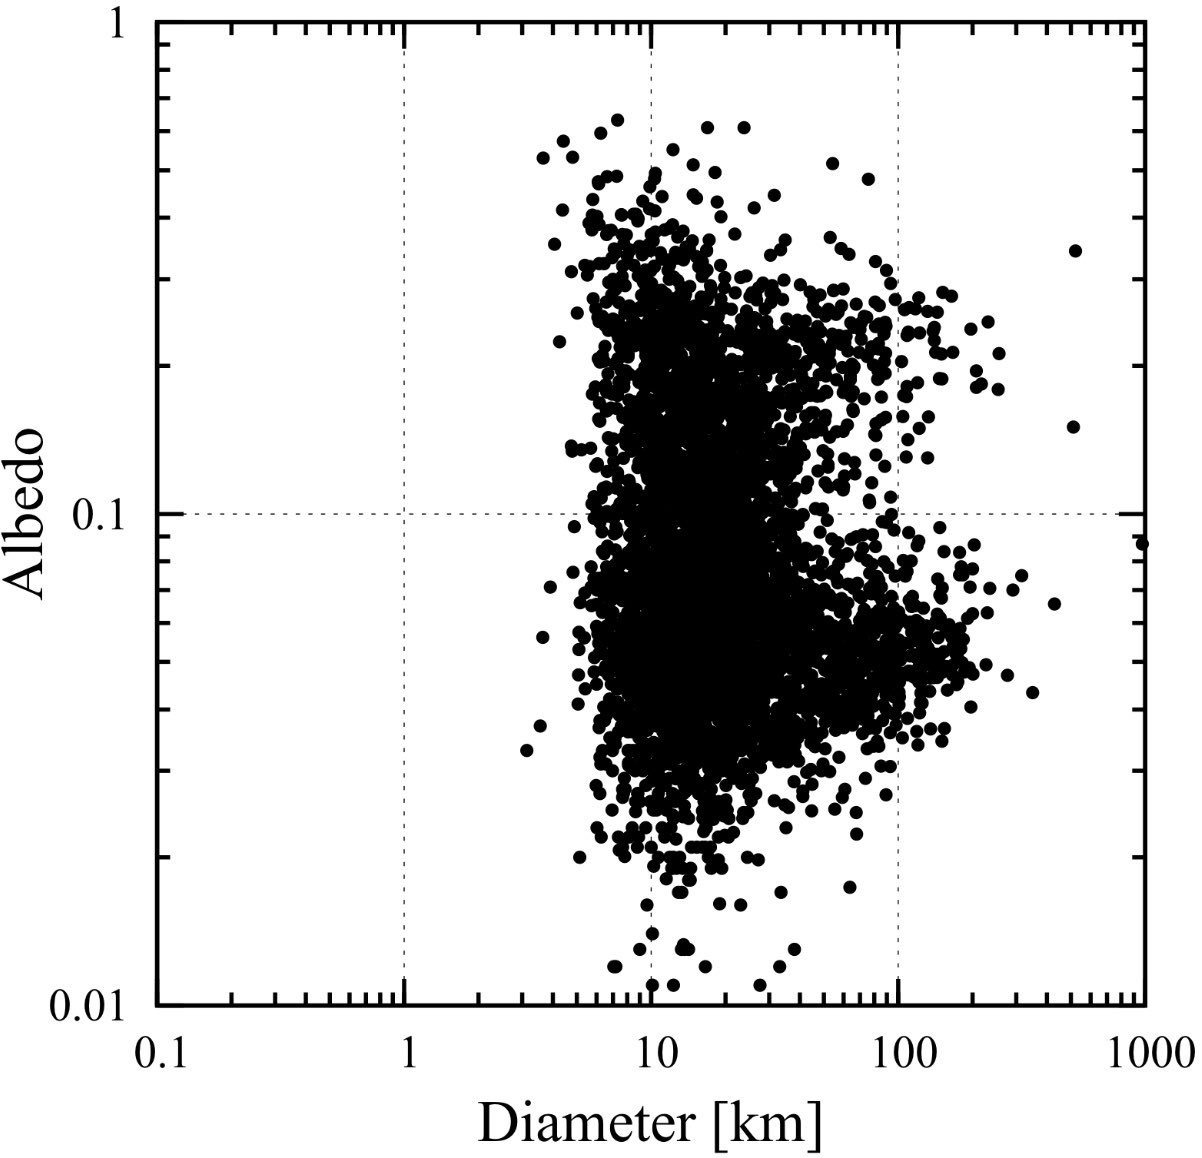
\includegraphics[keepaspectratio,angle=-90,origin=c,width=0.95\textwidth]{A-D}\end{figure}
\end{column} \end{columns}
\begin{block}{Classificazione dinamica}
\begin{itemize}
\item Fascia principale: tra Marte (perielio \SI{1.66}{\astronomicalunit}) e Giove.
\item Rapido spopolamento man mano che ci si avvicina a Giove.
\item Lacune di Kirkwood: per valori del semi-asse maggiore risonanti con quello di Giove.
\item grouping of proper elements: $\bar{e}\approx0.13$, $\bar{i}\approx\deg{7}$.
\end{itemize}
\end{block}
\end{frame}

\begin{wordonframe}{Classificazione asteroidi: orbita, spin, albedo, etc}
Sono la principale sorgente di meteoriti.
Orbite comprese tra Marte e Giove. Il primo \'e 1Ceres, diametro circa \SI{1000}{\kilo\meter}.
Da Terra si vedono come sorgenti puntiformi. Forma, dimensioni e caratteristiche superficiali: tecniche interferometriche e fenomeni di occultamento.
La spettro di riflessione \'e vario: dipende dalle caratteristiche chimiche e fisiche della superficie.
Paucity of asteroid in mean motion/secular resonance with planets.
Disruptive collisions (mean $v_r$ circa 4 $v_e$(ceres)$\approx\SI{5}{\kilo\meter\per\second}$).
\end{wordonframe}

\begin{frame}{famiglie collisionali}
\begin{figure}[!ht]
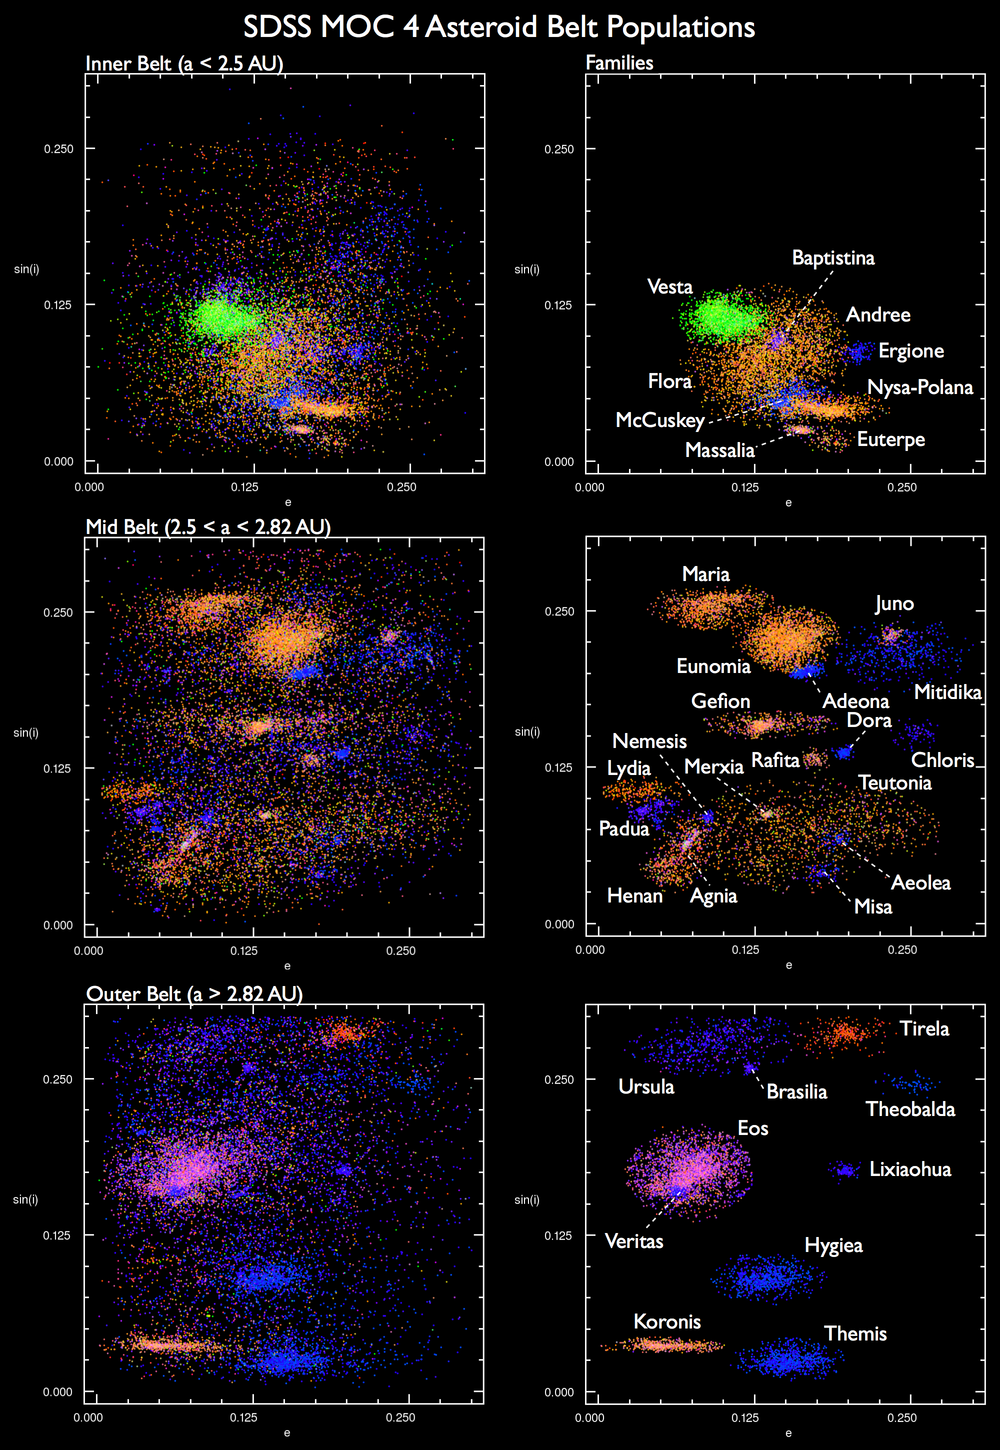
\includegraphics[keepaspectratio,width=0.6\textwidth]{Asdss}
\end{figure}
\begin{block}{Evoluzione}
\begin{itemize}
\item Collisioni: disruptive collisions, inject in resonannt regions, A. families,
\item Resonances: ejection solar system, NEO.
\end{itemize}
\end{block}
\end{frame}

\begin{wordonframe}{famiglie collisionali}

\end{wordonframe}

\begin{frame}{size distribution}
\begin{figure}[!ht]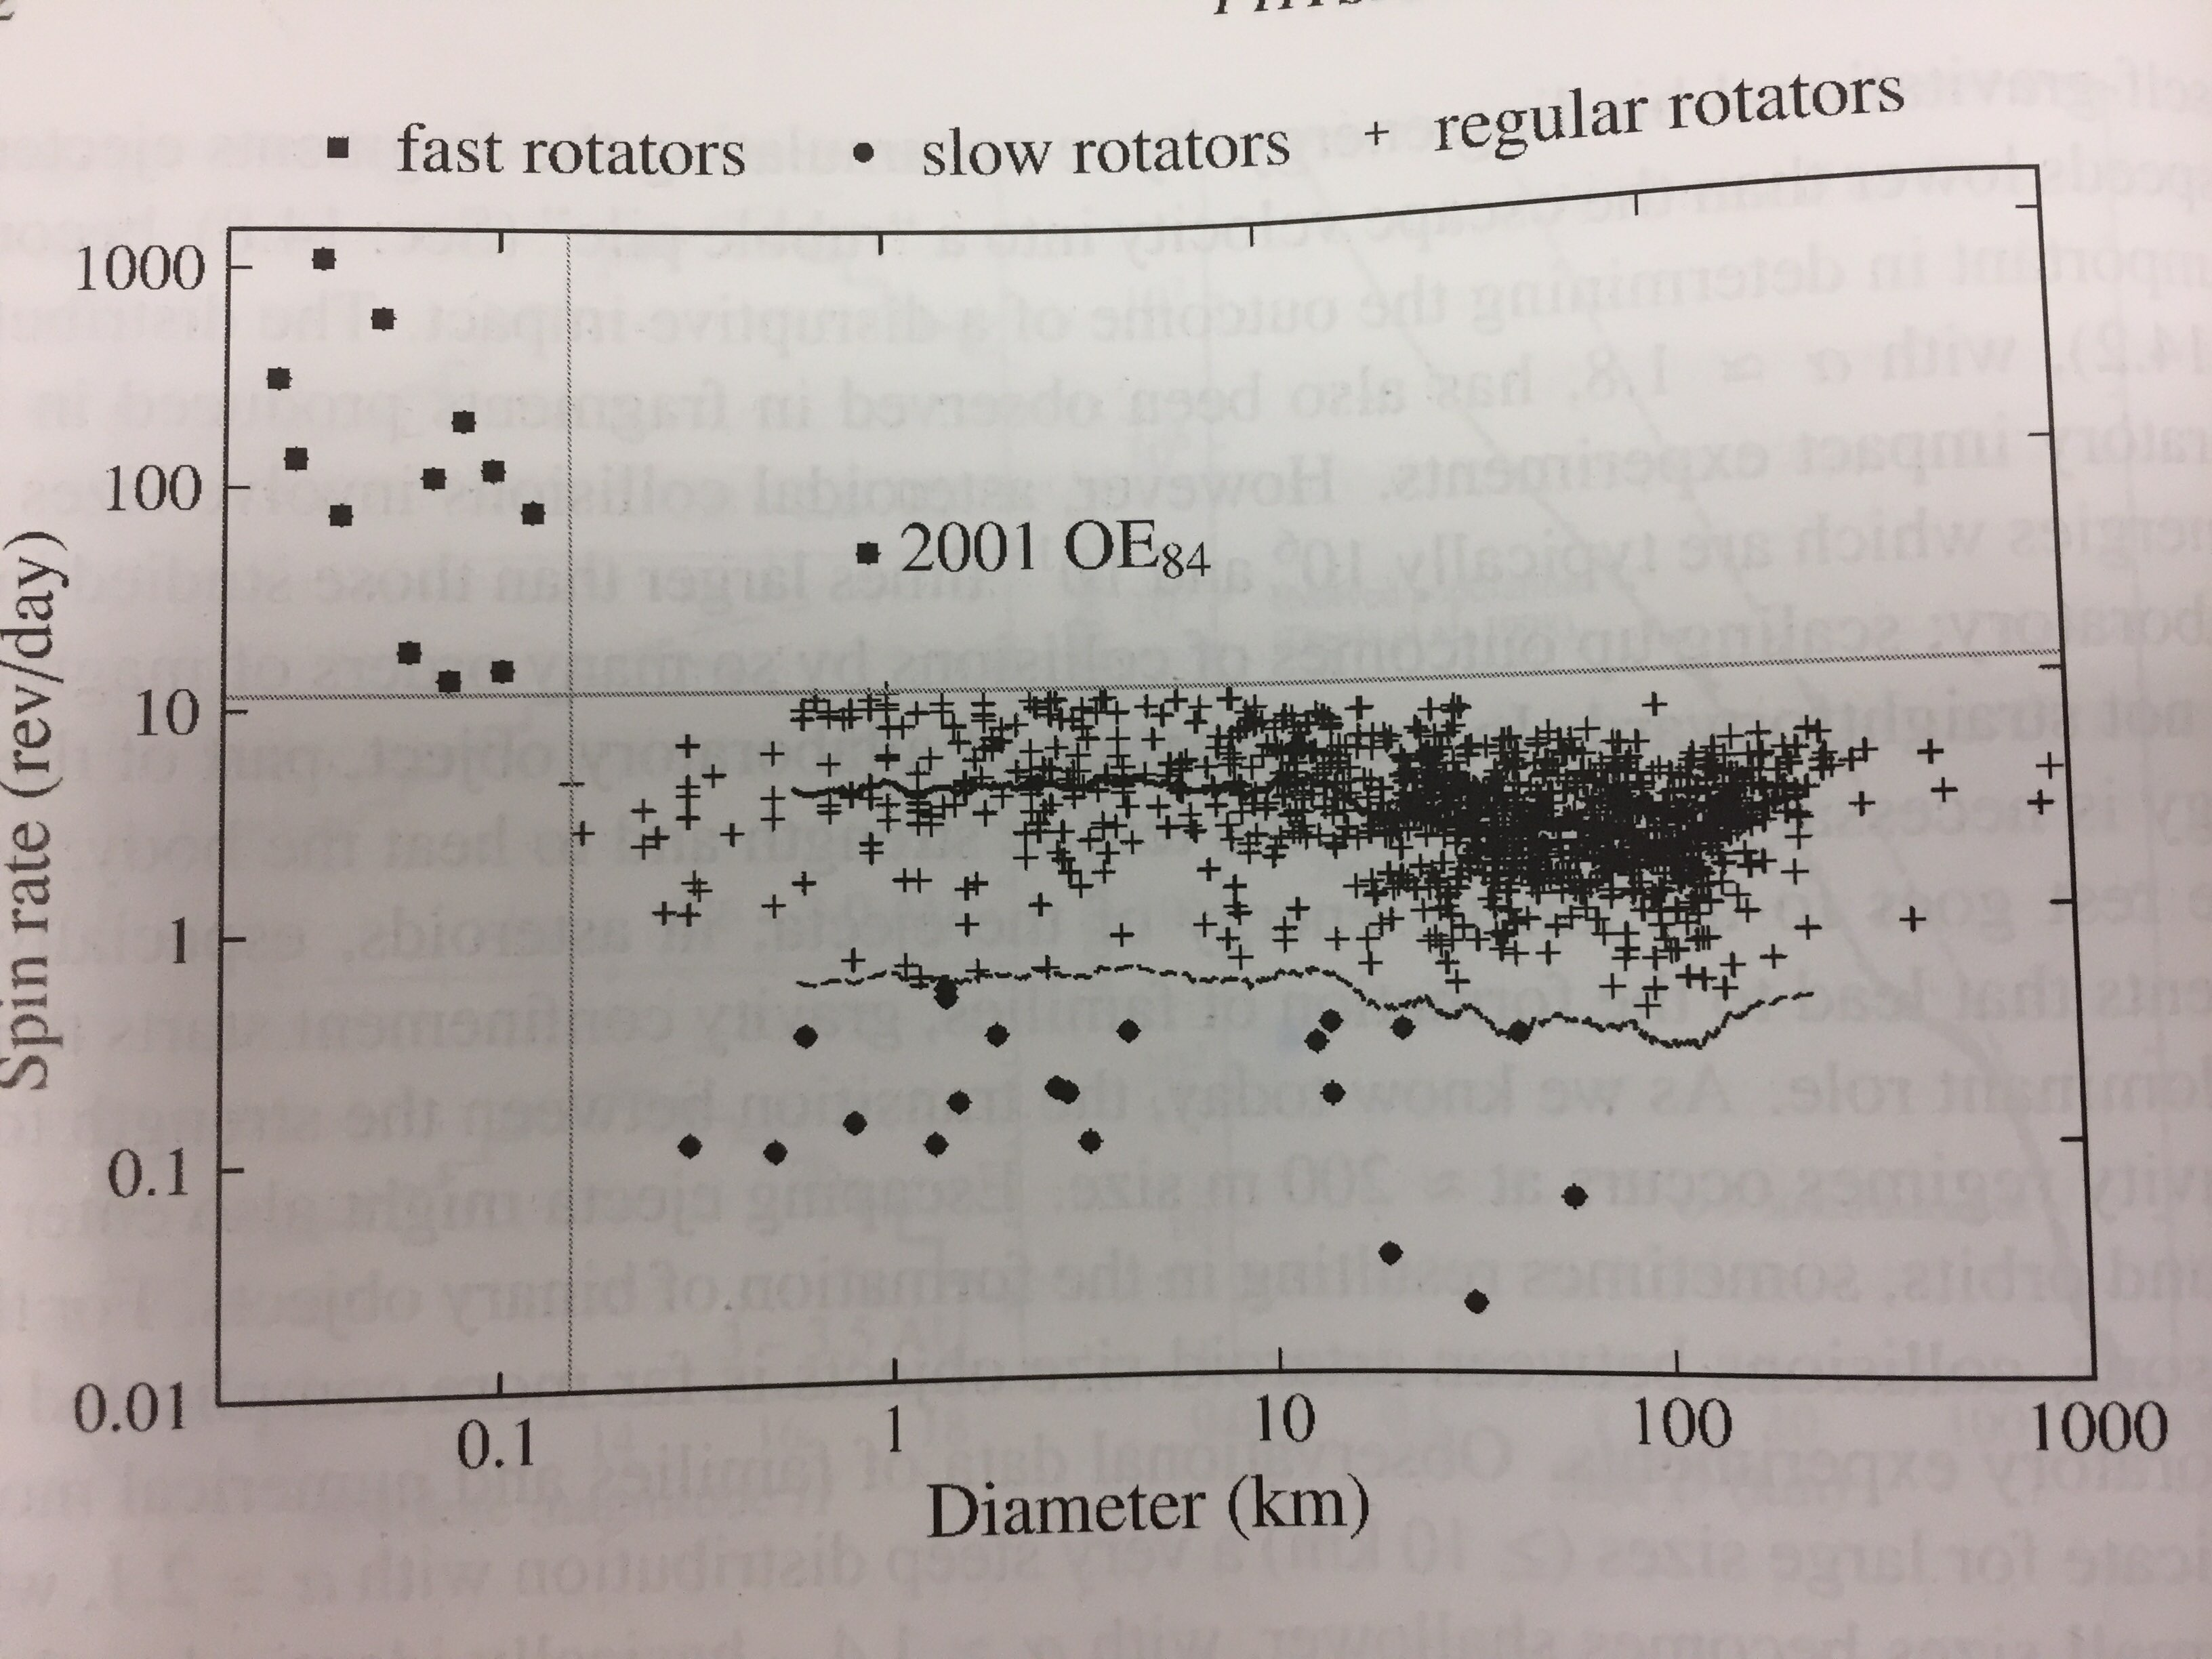
\includegraphics[keepaspectratio,width=0.6\textwidth]{spinD}
\end{figure}
$dN\propto m\expy{-\alpha}\,dm\propto D\expy{\beta}\,dD$
\end{frame}

\begin{wordonframe}{Distribuzione di massa A.}
\begin{block}{Collisional cascade (Dohnanyi '70, modello semplificato)}

\end{block}
\end{wordonframe}

\begin{frame}{NEO}
Orbita pi\'u interna, incrocia anche l'orbita della Terra.
\end{frame}

\begin{frame}{Meteoriti}

\end{frame}

\begin{wordonframe}{spettro di massa dei meteoriti}

\end{wordonframe}

\subsection{Kuiper, TNO, comets}

\begin{frame}{Reservoir di corpi}

\end{frame}

\begin{wordonframe}{Jupiter class comets}

\end{wordonframe}

\begin{frame}{Resonanze in TNO}
The orbits of Pluto and the plutinos are stable, despite crossing that of the much larger Neptune, because they are in a 2:3 resonance with it.
In the rings of Saturn, the Cassini Division is a gap between the inner B Ring and the outer A Ring that has been cleared by a $2:1$ resonance with the moon Mimas. (More specifically, the site of the resonance is the Huygens Gap, which bounds the outer edge of the B Ring.)
    In the rings of Saturn, the Encke and Keeler gaps within the A Ring are cleared by 1:1 resonances with the embedded moonlets Pan and Daphnis, respectively. The A Ring's outer edge is maintained by a destabilizing $7:6$ resonance with the moon Janus.
Most bodies that are in resonance orbit in the same direction; however, a few retrograde damocloids have been found that are temporarily captured in mean-motion resonance with Jupiter or Saturn. Such orbital interactions are weaker than the corresponding interactions between bodies orbiting in the same direction.
\end{frame}

\subsubsection{Troiani.}

Sono oggetti che hanno lo stesso semi-asse di Giove ma spostati di \ang{+-60} nell'orbita cio\'e nei punti Lagrangiani.

\subsubsection{Comete.}
Orbite eccentriche.

Il cambiamento delle loro propriet\'a dipende dalla distanza dal Sole: ricche di sostanze volatili

Originaria di una fascia esterna di corpi minori compresa tra asteroidi e TNO, in seguito a incontri ravvicinati con corpi maggiori si sono spostate in orbite che raggiungono all'afelio i confini del sistema solare (Nube di Oort approx \SI{e5}{\astronomicalunit}: quando diventa prevalente l'attrazione delle stelle vicine).

\subsubsection{Centauri.}

Centauri: orbite comprese tra Giove e Nettuno. La zona \'e dinamicamente instabile e porta in orbite cometaria.

\subsubsection{Trans-Neptunian object: Fascia di Kuiper-Edgeworth.}

Oltre Nettuno di hanno i TNO.

Un sottogruppo dei TNO, i plutini, sono in risonanza $3:2$ con Nettuno (come Plutone).

\subsection{Search motivation}

\begin{itemize}
\item Why acretional formation of solar system planet objects should stop at Neptuno's distance.
\item The jupiter family comets are almost on planar orbits with low inclination on ecliptic plane (plane of solar system). This is inesplicable if the source is far away and isotropic, so we may may postulate a a disc of cometary object beyond Neptun.
\end{itemize}

\subsection{Comets}

\subsection{Asteroids}

\subsection{Short summary}
\begin{itemize}
\item Originate from primitive bodies: TNO, comets and asteroids.
\item Span 20 order of magnitude in mass
\item Observed ground or space based optically or IR: reflected solar light or thermal emission by small interplanetary dust arranged in a disk like structure on the ecliptic plane.
Zodiacal light is caused by reflected light at large angle, false corona light is attributed to small angle diffractive scattering.
\end{itemize}


